\documentclass[french]{beamer}
\usetheme{Warsaw}
\usepackage{lmodern}
\usepackage[utf8]{inputenc}
\usepackage[T1]{fontenc}
\usepackage{babel}
\usepackage{color}
\usepackage{listings}
\usepackage{booktabs}
\usepackage{amsmath,amsthm,amssymb,graphicx,mathrsfs}
%\usepackage[hmargin={3.5cm,3.5cm},top=4cm,bottom=4cm]{geometry} %problem...

\newcommand{\vb}[1]{\mathbf{#1}}
\newcommand{\V}[1]{\textnormal{#1}}
\newcommand{\dd}[0]{\textrm{d}}
\newcommand{\bra}[1]{\langle#1 |}
\newcommand{\ket}[1]{| #1 \rangle}
\newcommand{\vdot}[0]{\boldsymbol\cdot}

\setbeamertemplate{footline}[frame number]{}
\setbeamertemplate{navigation symbols}{}
\setbeamertemplate{caption}[numbered]

\RequirePackage{cleveref}
\newtheorem{theoreme}{Théorème}
%%%%%%%%%%%%%%%%%%%%%%%%%%%%
\lstset{%
  backgroundcolor=\color{white},   % choose the background color; you must add \usepackage{color} or \usepackage{xcolor}
  basicstyle=\small,        % the size of the fonts that are used for the code
  commentstyle=\color{blue},    % comment style
  extendedchars=true,              % lets you use non-ASCII characters; for 8-bits encodings only, does not work with UTF-8
  keepspaces=true,                 % keeps spaces in text, useful for keeping indentation of code (possibly needs columns=flexible)
  keywordstyle=\color{red},       % keyword style
  language=Fortran,                 % the language of the code
  rulecolor=\color{black},         % if not set, the frame-color may be changed on line-breaks within not-black text (e.g. comments (green here))
  showspaces=false,                % show spaces everywhere adding particular underscores; it overrides 'showstringspaces'
  showstringspaces=false,          % underline spaces within strings only
  showtabs=false,                  % show tabs within strings adding particular underscores
  stringstyle=\color{green},     % string literal style
  tabsize=2,                       % sets default tabsize to 2 spaces
  frame=single
}



%%%%%%%%%%%%%%%%%%%%%%%%%%%%%%%%%%%%%%%%%%%%%%%%%%%%%%%%%%%%%%%%%%%%%%%%
\title{Propriétés spectroscopiques de l'oxalate de calcium}
\author{En-Hung CHAO, Honghao LI}
\institute{École Polytechnique}
\date{\today}
%%%%%%%%%%%%%%%%%%%%%%%%%%%%%%%%%%%%%%%%%%%%%%%%%%%%%%%%%%%%%%%%%%%%%%%%
%%%%%%%%%%%%%%%%%%%%%%%%%%%%%%%%%%%%%%%%%%%%%%%%%%%%%%%%%%%%%%%%%%%%%%%%
\begin{document}
\graphicspath{{../images/}}

\begin{frame}
\titlepage%
\end{frame}
%%%%%%%%%%%%%%%%%%%%%%%%%%%%%%%%%%%%%%%
%%%%%%%%%%%%%%%%%%%%%%%%%%%%%%%%%
\begin{frame}
\frametitle{Plan de présentation}
\framesubtitle{}
\begin{enumerate}
\item Introduction
\item Études de l'état fondamental
\item Études des états excités
\item Conclusion
\end{enumerate}
\end{frame}
%%%%%%%%%%%%%%%%%%%%%%%%%%%%%%%%%%%%%%%

%%%%%%%%%%%%%%%%%%%%%%%%%%%%%%%%%%%%%%%%%%%%%%%%%%%%%%%%%%%%%
\begin{frame}
\frametitle{Introduction}
\framesubtitle{Études spectroscopiques}
\begin{columns}
  \begin{column}{0.5\textwidth}
    \begin{figure}[!h]
    \centering
    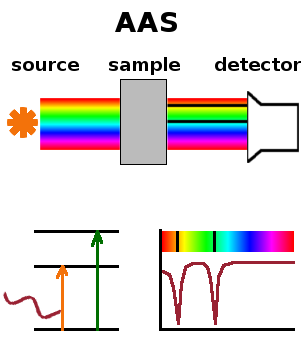
\includegraphics[width=0.6\textwidth]{absorption}
    \vspace{3em}
    \caption{Absorption}
    \end{figure}
  \end{column}
  \begin{column}{0.5\textwidth}
    \begin{figure}[!h]
    \centering
    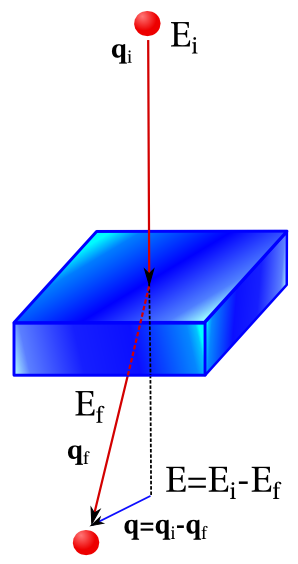
\includegraphics[width=0.5\textwidth]{eels}
    \caption{Dispersion et moment tranféré}
    \end{figure}
  \end{column}
\end{columns}
\end{frame}
\newpage

\begin{frame}
\frametitle{Introduction}
\framesubtitle{Calcul \textit{ab initio}}
\begin{itemize}
  \item Équation de Schrödinger
  \item Potentiel coulombien
\end{itemize}
\end{frame}
\newpage

\begin{frame}
\frametitle{Introduction}
\framesubtitle{Oxalade de Calcium}
\begin{itemize}
  \item Très présent dans la nature.
  \item En médicine et biologie: Le sang, les calculs rénaux.
  \item Expériences en cours au Laboratoire de la Physique des Solides (LPS) à Orsay.
\end{itemize}
\begin{figure}[!h]
  \centering
  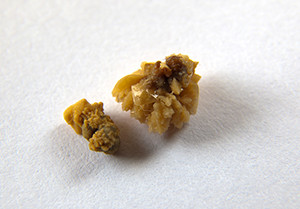
\includegraphics[height=0.4\textheight]{calcium-oxalate-kidney-stone}
  \caption{Calculs rénaux, communément appelés ``pierres aux reins''}
\end{figure}
\end{frame}
\newpage

\begin{frame}
\frametitle{Études de l'état fondamental}
\framesubtitle{Structure de l'oxalate de calcium}
La cellule élémentaire de l'oxalate de calcium ($CaC_2O_4$) contient 28 atomes et est de structure monoclinique.
\begin{figure}[!h]
  \centering
  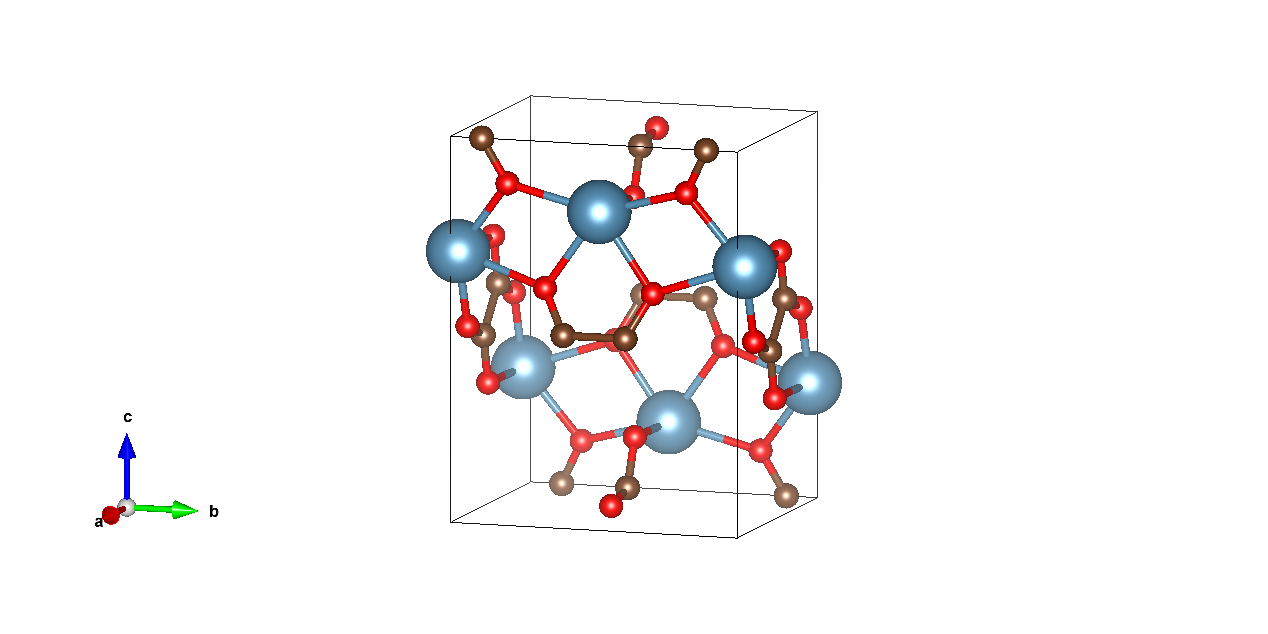
\includegraphics[height=0.4\textheight]{co_structure}
  \caption{La cellule élémentaire de l'oxalate de calcium avec $Ca$ en bleu, $O$ en rouge et $C$ en marron.}\label{BrillouinZone}
\end{figure}
\end{frame}
\newpage

\begin{frame}
\frametitle{Études de l'état fondamental}
\framesubtitle{}
Fonction d'onde du système:
\begin{equation*}
  \Psi(\vb{r}_1, \vb{r}_2, \ldots, \vb{r}_N)
\end{equation*}
où $N=256$ pour le cas de $CaC_2O_4$.

$\Rightarrow $ l'espace de dimension $768$ à considérer.

\end{frame}
\newpage
%%%%%%%%%%%%%%%%%%%%%%%%%%%%%%%%%%%%%%%%%%%%5555
\begin{frame}
\frametitle{Études de l'état fondamental}
\framesubtitle{Théorie de la fonctionnelle de la densité, DFT en anglais}
\begin{theoreme}[Hohenberg-Kohn]
  L'espérance d'une observable dans l'état fondamental est une fonctionnelle unique
  de la densité d'électrons.
\end{theoreme}

\begin{theoreme}[Kohn-Sham]
  Pour tout système qui contient des termes d'interaction entre électrons,
  il existe un système auxiliaire non-interagissant ayant la même densité d'électrons.
\end{theoreme}

\textbf{Conclusion} la résolution d'un système à plusieurs corps se réduit à la recherche de la fonction de la densité d'un système d'électrons non-interagissant.
\end{frame}
\newpage
%%%%%%%%%%%%%%%%%%%%%%%%%%%%%%%%%%%%%%%%%%%%%%
\begin{frame}
\frametitle{Études de l'état fondamental}
\framesubtitle{DFT}
Le nouveau système d'équations à considérer

\begin{equation*}
  (-\frac{1}{2}\nabla_i + V_{tot}[n](\textbf{r}))\phi_i(\textbf{r}) = \epsilon_i\phi_i(\textbf{r})
\end{equation*}
avec

\begin{equation*}
  V_{tot}(\textbf{r}) = \underbrace{V_{ext}(r)}_\text{ions}
  + \underbrace{\int \dd \textbf{r}' \frac{n(\textbf{r}')}{|\textbf{r} - \textbf{r}'|}}_\text{potentiel de Hartree}
  + \underbrace{V_{xc}([n], \textbf{r})}_\text{échange-corrélation}
\end{equation*}
\textbf{Remarque} un terme d'échange-corrélation apparaît

$\Rightarrow$ Approximations nécesitées (avec l'approximation des gradients généralisée, GGA en anglais)

Solution du système d'équations: $\phi_i(\vb{r})$. Processus itératif:
\begin{equation*}
  n(\vb{r}) = \sum_i^N |\phi_i(\vb{r})|^2
\end{equation*}
\end{frame}
\newpage
%%%%%%%%%%%%%%%%%%%%%%%%%%%%%%%%%%%%%%%%%%%%%%%%%%%%%%%%%%%%%
\begin{frame}
\frametitle{Études de l'état fondamental}
\framesubtitle{Calculs numériques}
\begin{itemize}
  \item Réalisé avec le code d'\textit{Abinit}.
  \item Fonctionnement:
    Théorème de Bloch
    \begin{equation*}
      \phi_{n,\textbf{k}_i}
      = e^{i\textbf{k}_i\cdot\textbf{r}} u_{n,\textbf{k}_i}(\textbf{r})
      = \frac{1}{\sqrt{\Omega_{maille}}}e^{i\textbf{k}_i\cdot\textbf{r}}\sum_{\textbf{G}} c_{n,\textbf{k}_i}(\textbf{G})e^{i\textbf{G}\cdot\textbf{r}}
    \end{equation*}
  \item Réduction de la dimension de la base d'ondes planes en définissant une énergie de seuil $E_{cut}$:
    \begin{equation*}
      \frac{1}{2}|\textbf{k}+\textbf{G}|^2 \leq E_{cut}
    \end{equation*}

  \item Résultat obtenu:

    La densité d'électrons $n(\vb{r})$ dans l'état fondamental

    $\Rightarrow$ l'espérance d'observable: e.g.\ l'énergie totale

\end{itemize}

\end{frame}

%%%%%%%%%%%%%%%%%%%%%%%%%%%%%%%%%%%%%%%%%%%%%%%%
\begin{frame}
\frametitle{Études de l'état fondamental}
\framesubtitle{Convergence en énergie de seuil du système}
\begin{figure}[!h]
    \centering
    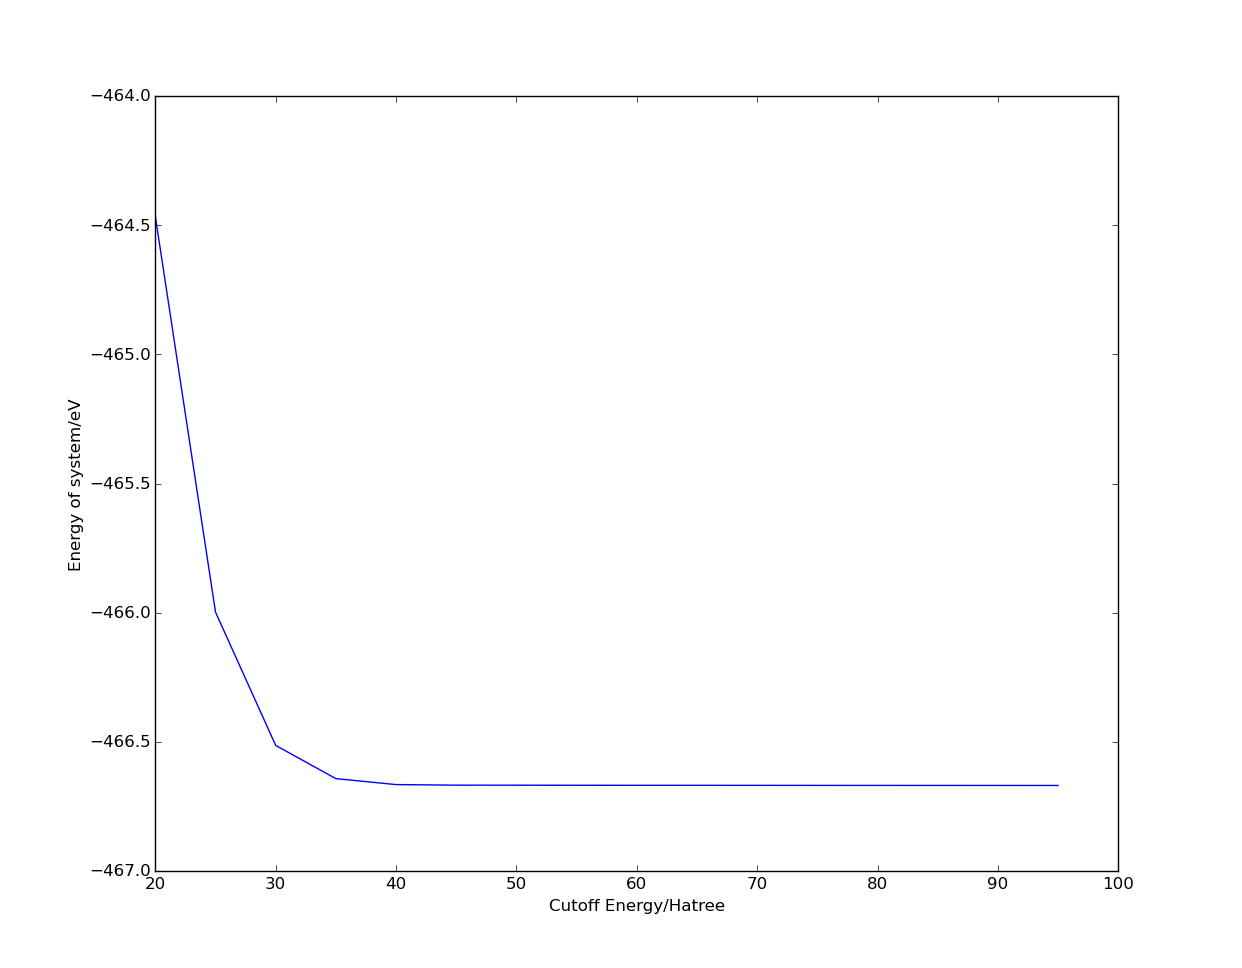
\includegraphics[width=8cm]{E_cut}
    \caption{L'énergie totale du système (en eV) en fonction de l'énergie de seuil (en Hartree). $E_{\V{cut}} = 40\ \V{Hartree}\sim 35000$ ondes planes }\label{fig-Ecut}
\end{figure}
\end{frame}

%%%%%%%%%%%%%%%%%%%%%%%%%%%%%%%%%%%%%%%%%%%%%%%%
\begin{frame}
\frametitle{Études de l'état fondamental}
\framesubtitle{Convergence de l'échantillonnage}

\begin{equation*}
  n(\vb{r}) = \sum_{n, \vb{k}}^{\V{occ}} |\phi_{n, \vb{k}}(\vb{r})|^2
\end{equation*}

\begin{itemize}
\item Calul discrétisé dans l'espace réciproque $\Longrightarrow$ échantillonnage de la première zone de Brillouin
\item Choix d'échantillonnage pertinents (respectant les symétries du problème)

\end{itemize}
\begin{table}[ht]
  \caption{Énergie totale du système en fonction du nombre de points-$\textbf{k}$}
  \centering
  \begin{tabular}{c c}
    \toprule
    Nombre de points-$\textbf{k}$  &  $E_{tot}$ à la convergence (Hartree)
    \\
    \midrule
    16    &  -466.66501448840
    \\
    28    &  -466.66501224916
    \\
    40    &  -466.66501098806
    \\
    \bottomrule
  \end{tabular}
\end{table}

\end{frame}

%%%%%%%%%%%%%%%%%%%%%%%%%%%%%%%%%%%%%%%%%%%%%%%%
\begin{frame}
\frametitle{Études des états excités}
\framesubtitle{TDDFT}
\begin{itemize}
\item Théorie de la fonctionelle de la densité dépendante du temps
\item $\vb{E} = \epsilon^{-1}\vb{D}$
\item Absorption et spectre de pertes en énergie (EELS)
\begin{equation*}
  \textrm{Abs} = \Im\{\epsilon(\omega, \textbf{q})\},
  \quad
  \textrm{EELS} = -\Im\{\epsilon^{-1}(\omega, \textbf{q})\}.
\end{equation*}

\begin{figure}[!h]
  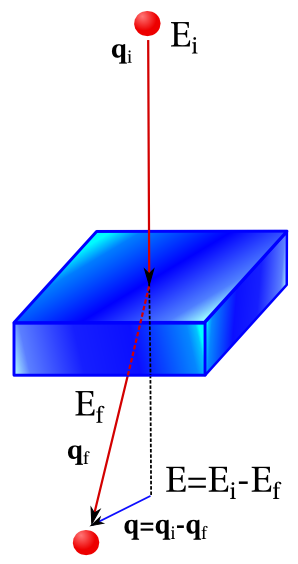
\includegraphics[width=0.2\textwidth]{eels}
  \caption{Dispersion et moment transféré}
\end{figure}
\end{itemize}
\end{frame}

%%%%%%%%%%%%%%%%%%%%%%%%%%%%%%%%%%%%%%%%%%%%%%%%
\begin{frame}
\frametitle{Études des états excités}
\framesubtitle{TDDFT}
\begin{itemize}
\item Relation entre $\chi$ et $\epsilon$:
\begin{equation*}
  \epsilon^{-1} = 1+ v\chi.
\end{equation*}
\item Fonctions de polarisation:
\begin{equation*}
\begin{split}
\delta n(\vb{r}, \omega) &= \int \dd{\vb{r}'} \chi(\vb{r}, \vb{r}', \omega)\delta V_{\V{ext}}(\vb{r}',\omega)\\
\end{split}
\end{equation*}
\item Relation entre $\chi$ et $\chi^0$:
\begin{equation*}
\chi = \chi^0 ( 1 + (v+f_{\textrm{xc}})\chi)
\end{equation*}
$\Longrightarrow$ terme d'échange-corrélation à approximer,  avec la \textit{Random Phase Approximation} (RPA) et la \textit{Adiabatic Local Density Approximation} (ALDA) dans notre cas
\end{itemize}
\end{frame}
\newpage

\begin{frame}[shrink=20]
\frametitle{Études des états excités}
\framesubtitle{TDDFT}
\begin{equation*}
  \chi^0(q, \vb{G}, \vb{G}', \omega) = \frac{2}{\Omega}\sum_{v,c,\vb{k}}(f_{c,\vb{k}+\vb{q}} - f_{v,\vb{k}}) \frac{\bra{v, \vb{k}}e^{-i(\vb{q}+\vb{G})\vdot\vb{r}} \ket{c , \vb{k}+\vb{q}}\bra{c, \vb{k}+\vb{q}} e^{-i(\vb{q}+\vb{G}')\vdot\vb{r}} \ket{v , \vb{q}}}{\omega - (\epsilon_{c, \vb{k}+\vb{q}} - \epsilon_{v,\vb{k}}) + i\eta}
\end{equation*}
\begin{figure}[!h]
    \centering
    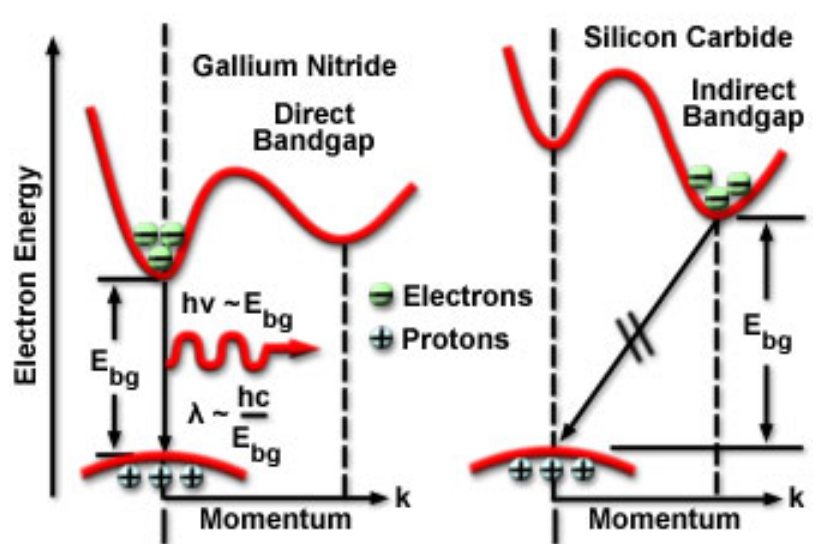
\includegraphics[width=8cm]{transition}
    \caption{Transitions entre bandes}
\end{figure}
\end{frame}
\newpage
%%%%%%%%%%%%%%%%%%%%%%%%%%%%%%%%%%%%%%%%%%%%%%%%
\begin{frame}
\frametitle{Études des états excités}
\framesubtitle{Convergence de l'échantillonnage}
À nouveau, il faut bien discrétiser l'espace de Fourier de la zone de Brillouin pour faire converger le calcul
\begin{figure}[!h]
    \centering
    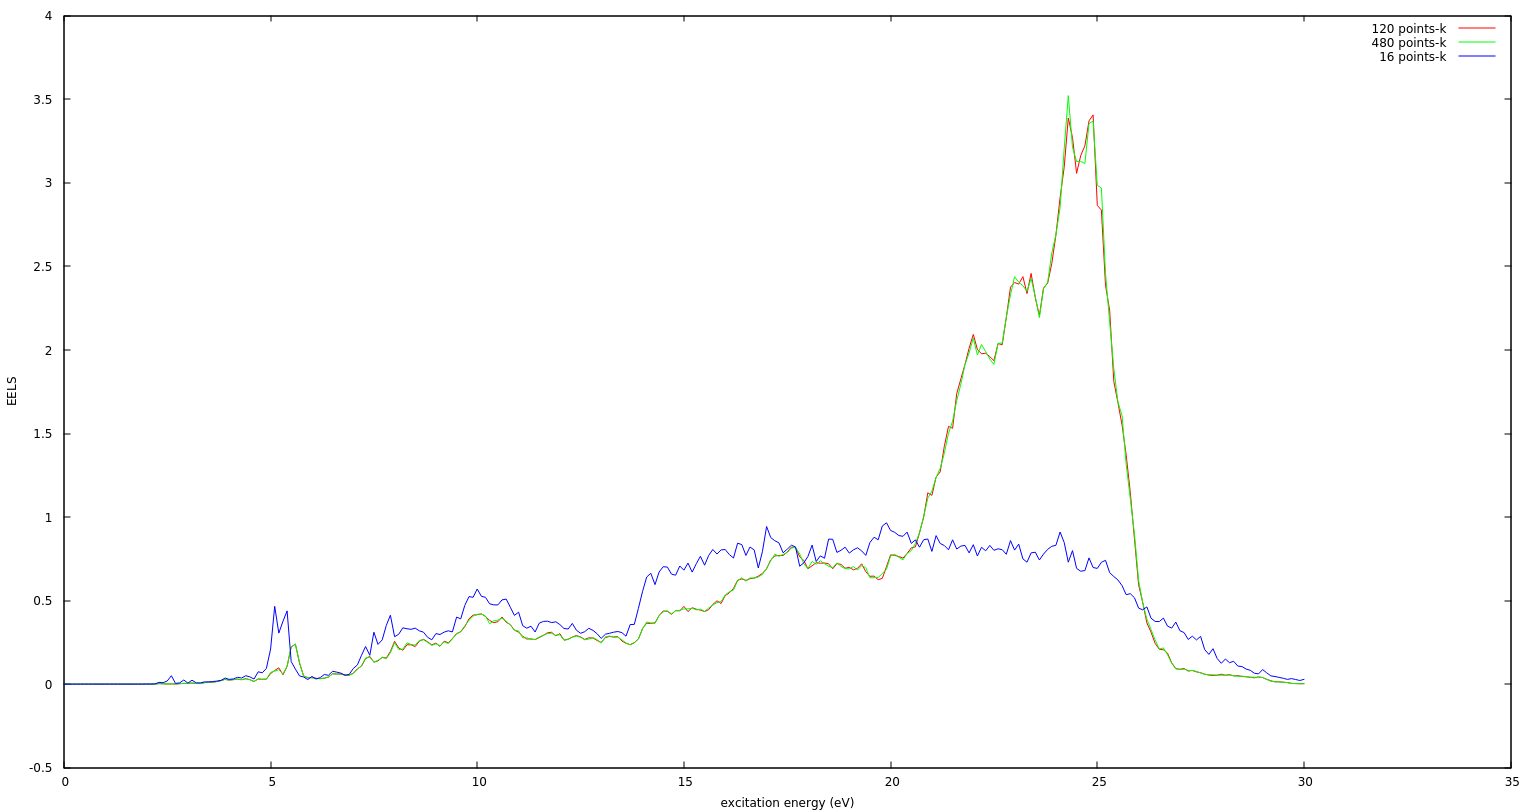
\includegraphics[width=8cm]{kpt_compare}
    \caption{Convergence pour des nombres de points-$\vb{k}$ différents}
\end{figure}

\end{frame}
%%%%%%%%%%%%%%%%%%%%%%%%%%%%%%%%%%%%%%%%%%%%%%%%%
\begin{frame}
\frametitle{Études des états excités}
\framesubtitle{Convergence avec les bandes}
\begin{columns}
  \begin{column}{\dimexpr0.3\paperwidth-10pt}
    \begin{figure}[!h]
    \centering
    \vspace{10pt}
    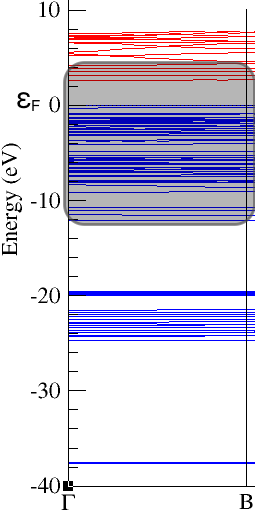
\includegraphics[width=0.9\textwidth]{band_structure_1}
    \caption{\centering Structure de bandes}\label{fig-band_1}
    \end{figure}
  \end{column}
  \begin{column}{\dimexpr0.7\paperwidth-10pt}
    \begin{figure}[!h]
   \centering
    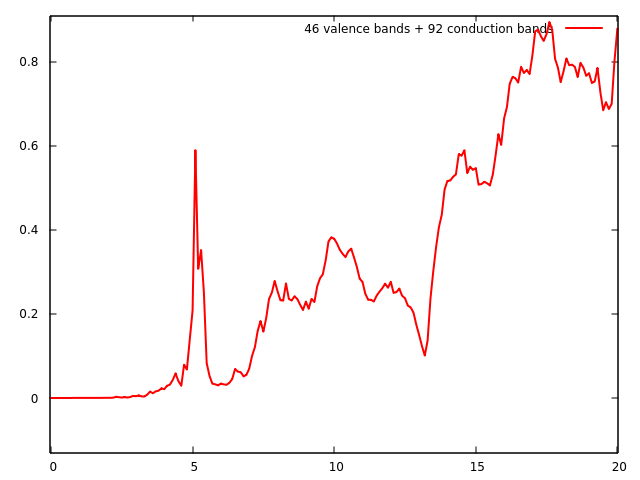
\includegraphics[width=\textwidth]{nbd_1}
    \caption{Convergence en bande}\label{fig-cv_nbd_1}
    \end{figure}
  \end{column}
\end{columns}

\end{frame}

\begin{frame}
\frametitle{Études des états excités}
\framesubtitle{Convergence avec les bandes}
\begin{columns}
  \begin{column}{\dimexpr0.3\paperwidth-10pt}
    \begin{figure}[!h]
    \centering
    \vspace{10pt}
    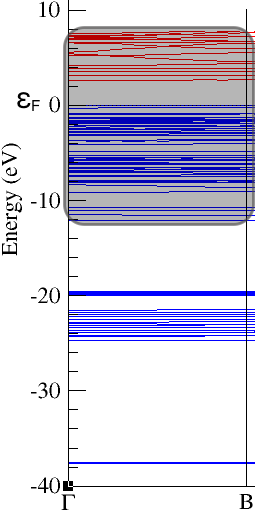
\includegraphics[width=0.9\textwidth]{band_structure_2}
    \caption{\centering Structure de bandes}\label{fig-band_2}
    \end{figure}
  \end{column}
  \begin{column}{\dimexpr0.7\paperwidth-10pt}
    \begin{figure}[!h]
    \centering
    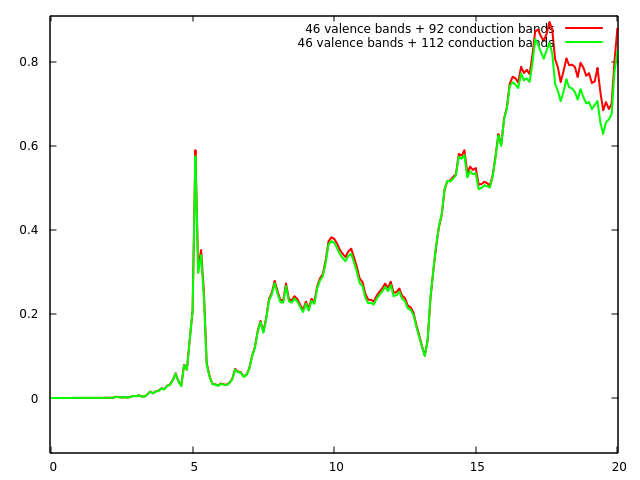
\includegraphics[width=\textwidth]{nbd_2}
    \caption{Convergence en bande}\label{fig-cv_nbd_2}
    \end{figure}
  \end{column}
\end{columns}

\end{frame}

\begin{frame}
\frametitle{Études des états excités}
\framesubtitle{Convergence avec les bandes}
\begin{columns}
  \begin{column}{\dimexpr0.3\paperwidth-10pt}
    \begin{figure}[!h]
    \centering
    \vspace{10pt}
    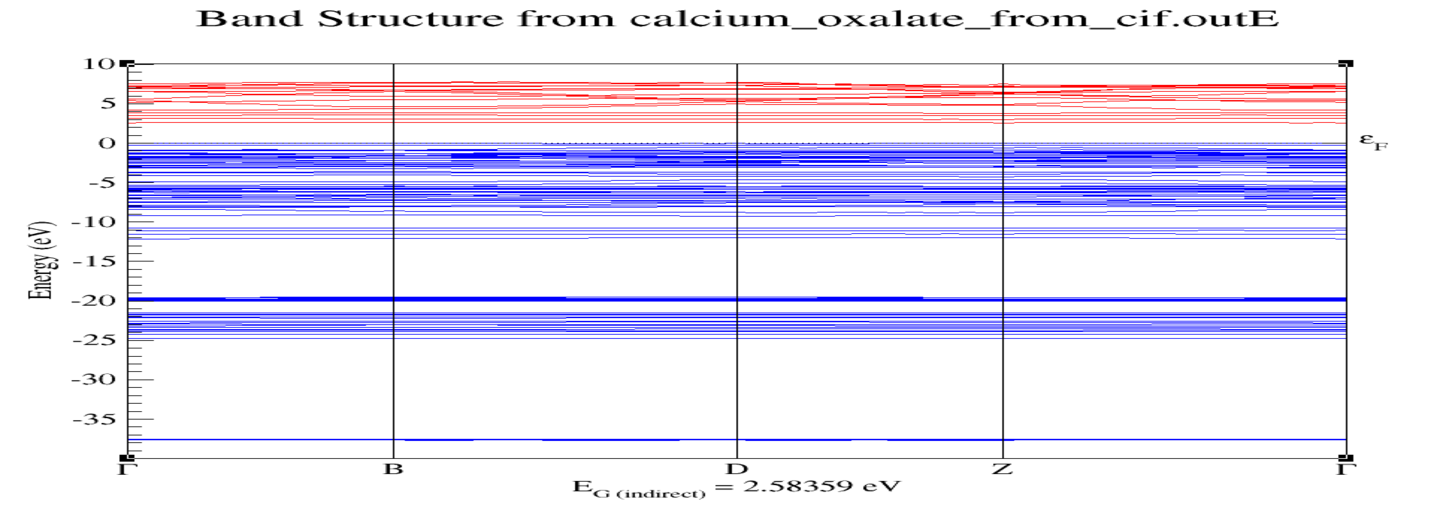
\includegraphics[width=0.9\textwidth]{band_structure}
    \caption{\centering Structure de bandes}\label{fig-band_3}
    \end{figure}
  \end{column}
  \begin{column}{\dimexpr0.7\paperwidth-10pt}
    \begin{figure}[!h]
    \centering
    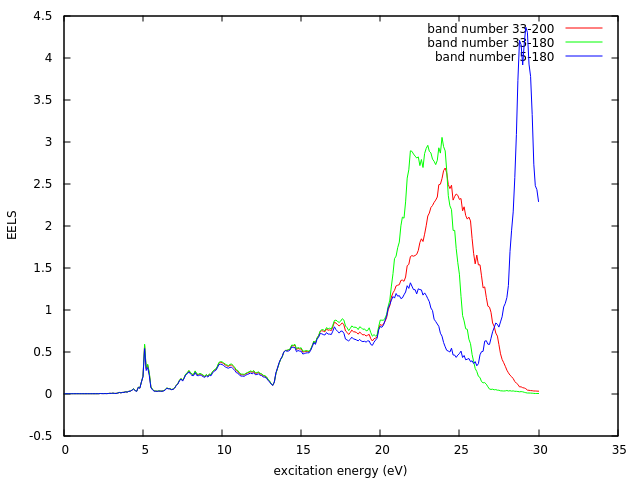
\includegraphics[width=\textwidth]{nbd_compare}
    \caption{Convergence en bande}\label{fig-cv_nbd_3}
    \end{figure}
  \end{column}
\end{columns}

\end{frame}
%%%%%%%%%%%%%%%%%%%%%%%%%%%%%%%%%%%%%%%%%%%%%%%%%


\begin{frame}
\frametitle{Études des états excités}
\framesubtitle{Comparaison entre RPA et ALDA}
\begin{figure}[!h]
    \centering
    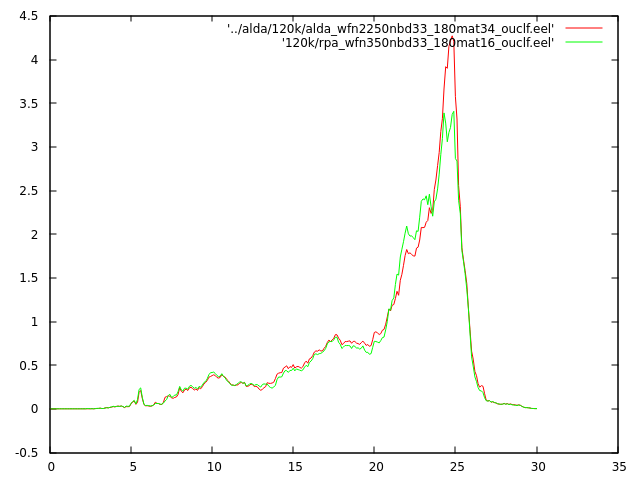
\includegraphics[width=8cm]{alda_vs_rpa}
    \caption{Approximation ALDA vs. RPA}\label{fig-alda_vs_rpa}
\end{figure}

\end{frame}
%%%%%%%%%%%%%%%%%%%%%%%%%%%%%%%%%%%%%%%%%%%%%%%%%
\begin{frame}
\frametitle{Études des états excités}
On a désormais:
\begin{itemize}
\item Convergence en échantillonnage
\item Les bandes nécessaires pour avoir la convergence
\item Bonne méthode d'approximation
\end{itemize}
$\Longrightarrow$ On peut passer à l'analyse du matériau
\end{frame}


%%%%%%%%%%%%%%%%%%%%%%%%%%%%%%%%%%%%%%%%%%%%%%%%%%%%
\begin{frame}
\frametitle{Analyse des résultats}
\framesubtitle{Anisotropie du système}
\begin{figure}[!h]
    \centering
    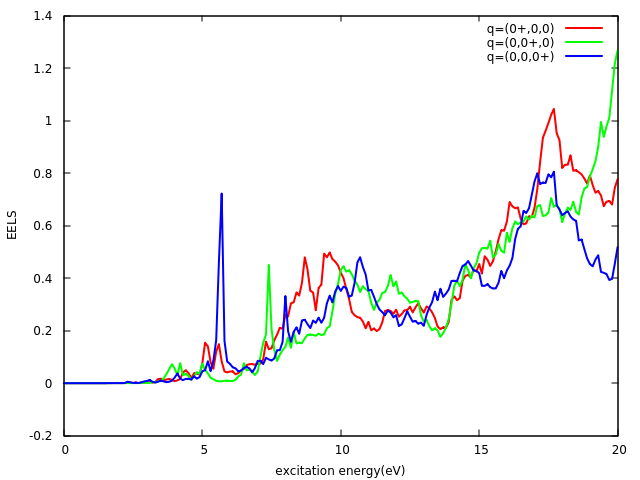
\includegraphics[width=8cm]{anisotropy}
    \caption{L'anisotropie du système}\label{fig-anisotropie}
\end{figure}

\end{frame}
%%%%%%%%%%%%%%%%%%%%%%%%%%%%%%%%%%%%%%%%%%%%%%%%%

\begin{frame}
\frametitle{Analyse des résultats}
\framesubtitle{EELS et la fonction diélectrique}
\begin{columns}
  \begin{column}{\dimexpr0.3\paperwidth-10pt}
  \centering
  $$
  \V{EELS}
  = \Im{(\epsilon^{-1})}
  $$
  $$
  = \frac{-\Im({\epsilon})}{\Re{(\epsilon)}^2 + \Im{(\epsilon)}^2}
  $$
  \end{column}
  \begin{column}{\dimexpr0.75\paperwidth-10pt}
        \begin{figure}[!h]
      \centering
      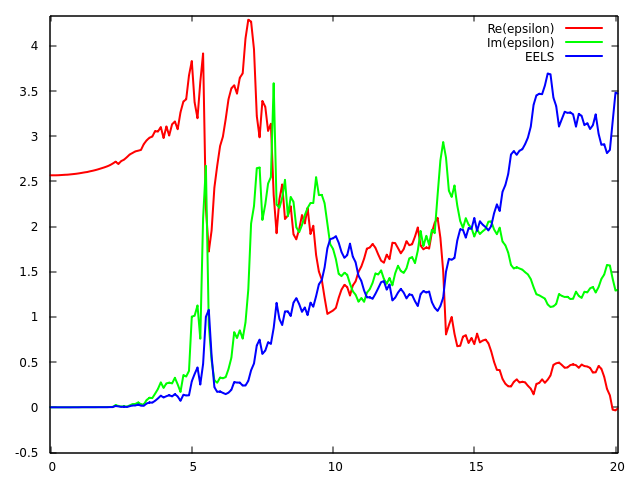
\includegraphics[width=8cm]{epsilon_compare}
      \caption{\centering Relation entre les parties réelle et imaginaire de la fonction diélectrique $\epsilon$ et EELS}\label{fig-epsilon_compare}
    \end{figure}
  \end{column}
\end{columns}

\end{frame}
%%%%%%%%%%%%%%%%%%%%%%%%%%%%%%%%%%%%%%%%%%%%%%%%%

\begin{frame}
\frametitle{Analyse des résultats}
\framesubtitle{Dispersion}
\begin{figure}[!h]
    \centering
    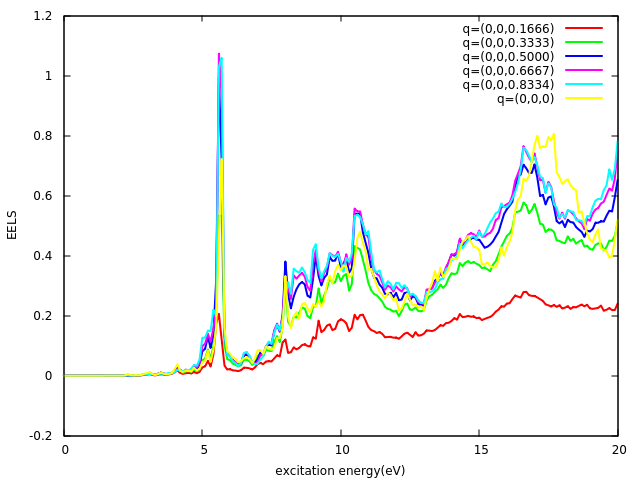
\includegraphics[width=8cm]{q6}
    \caption{EELS pour différents $\vb{q}$ dans la direction (0, 0, 1) dans la première zone de Brillouin}\label{fig-q6}
\end{figure}

\end{frame}
%%%%%%%%%%%%%%%%%%%%%%%%%%%%%%%%%%%%%%%%%%%%%%%%%
\begin{frame}
\frametitle{Analyse des résultats}
\framesubtitle{Dispersion}
\begin{figure}[!h]
    \centering
    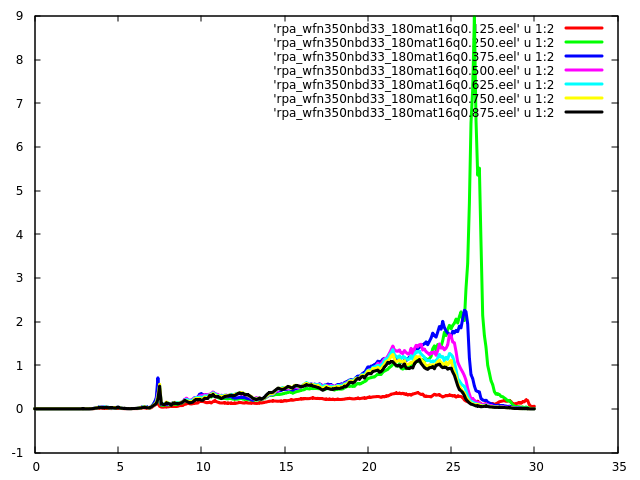
\includegraphics[width=8cm]{q8}
        \caption{EELS pour différents $\vb{q}$ dans la direction (0, 1, 0) dans la première zone de Brillouin}\label{fig-q8}
\end{figure}

\end{frame}
%%%%%%%%%%%%%%%%%%%%%%%%%%%%%%%%%%%%%%%%%%%%%%%%%
\begin{frame}
\frametitle{Analyse des résultats}
\framesubtitle{Dispersion}
\begin{figure}[!h]
    \centering
    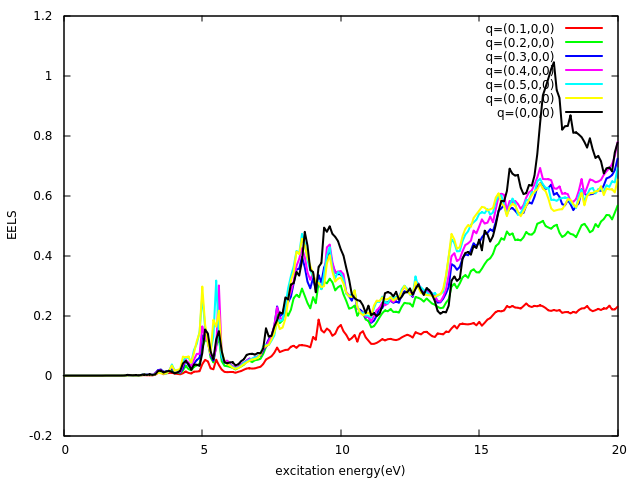
\includegraphics[width=8cm]{q10}
    \caption{EELS pour différents $\vb{q}$ dans la direction (1, 0,0) dans la première zone de Brillouin}\label{fig-q10}
\end{figure}
\end{frame}
%%%%%%%%%%%%%%%%%%%%%%%%%%%%%%%%%%%%%%%%%%%%%%%%%

\begin{frame}
\frametitle{Conclusion}
\begin{itemize}
  \item Conditions initiales $\rightarrow$ Études de convergence\\ $\rightarrow$ État fondamental $\rightarrow$ Études de convergence\\ $\rightarrow$ Dispersion, transition spectroscopique
  \item Prospective: états hydratés d'oxalate de calcium
  \item Projet de recherche en collaboration, discussion et réunion
  \item Compétences techniques: logiciel de visualisation, gestion de tâches de calcul sur les clusters
%\item Un premier aperçu sur le travail de recherche en laboratoire
%\item Fournir une référence aux expérimentateurs
%\item Perspective
\end{itemize}

\end{frame}
%%%%%%%%%%%%%%%%%%%%%%%%%%%%%%%%%%%%%%%%%%%%%%%%%

\end{document}
